\documentclass{article}
\usepackage{graphicx}
\usepackage[letterpaper, total={6.5in, 9in}]{geometry}
\usepackage{listings}

\usepackage{xcolor}

\definecolor{codegreen}{rgb}{0,0.6,0}
\definecolor{codegray}{rgb}{0.5,0.5,0.5}
\definecolor{codepurple}{rgb}{0.58,0,0.82}
\definecolor{backcolour}{rgb}{0.95,0.95,0.92}

\lstdefinestyle{mystyle}{
    backgroundcolor=\color{backcolour},   
    commentstyle=\color{codegreen},
    keywordstyle=\color{magenta},
    numberstyle=\tiny\color{codegray},
    stringstyle=\color{codepurple},
    basicstyle=\ttfamily\footnotesize,
    breakatwhitespace=false,         
    breaklines=true,                 
    captionpos=b,                    
    keepspaces=true,                 
    numbers=left,                    
    numbersep=5pt,                  
    showspaces=false,                
    showstringspaces=false,
    showtabs=false,                  
    tabsize=4
}

\lstset{style=mystyle}

\title{Project 1: RGB LED Cycler Solution}

\author{Braidan Duffy\thanks{B.S. Ocean Engineering 2021\\M.S. Ocean Engineering 2023}}

\date{May 24, 2022}

\begin{document}

\maketitle

\section*{Overview}

Students will have considered completing this project when they accomplish the following tasks:
\begin{enumerate}
    \item integrated an RGB LED and button input with their Arduino microcontroller
    \item implemented at least 3 functions within their code
        \subitem at least one of these functions must include a loop
    \item used a switch/case statement to switch between different functions
    \item uploaded a compressed file containing:
        \subitem a video of the project running with narration
        \subitem a neatly made and well-organized schematic
        \subitem a neatly organized Arduino code file
\end{enumerate}

\section*{Grading}
\begin{tabular}{ | p{1in} | p{1.75in} | p{1.75in} | p{1.75in} | }
    \hline
    \textbf{Category} & \textbf{No Credit} & \textbf{Half Credit} & \textbf{Full Credit} \\

    \hline
    Efficacy & 
    Student did not demonstrate their working project & 
    student demonstrated a working project, but it did not meet all of the requirements specified in the project handout & 
    student demonstrated a feature-complete project that accomplished all of the goals specified in the project handout \\
    \hline
    3 or more functions & 
    Student did not implement enough unique functions &
    &
    Student implemented enough functions \\
    \hline
    1 or more loops & 
    Student did not implement enough loops &
    &
    Student implemented enough loops \\
    \hline
    Schematic neatness & 
    Student did not provide a schematic, or it is illegible &
    Student provided a schematic, but it is difficult to read or understand &
    Student provided a schematic that is easy to read and understand \\
    \hline
    Mystery extra credit &
    Student did not request extra credit or reach the necessary thresholds & 
    Stduent successfully implemented either the debounced button input or unique RGB function or something equivalent and justified it adequately &
    Student successfully implemented both debounced button input or unique RGB function and/or something equivalent and justified it adequately \\

    \hline
\end{tabular}

\section*{Guide}

    \subsection*{Wiring the Breadboard}

    Students should begin the project by plugging in the RGB LED and button to the breadboard, and the GND pin of the Arduino to the negative (blue) rail of the breadboard; the Arduino's 5V pin should be connected to the positive (red) rail.
    They should then atttached 1k-ohm resistors to the three short pins of the LED and jump them across the middle of the breadboard, ensuring the two leads are \emph{not} within the same row and the resistor leads are \emph{not} touching.
    Each of the three resistors should then be connected to the Arduino according to the pinout in Figure \ref{fig:rgb_led_bb}.
    The longer pin (cathode) of the LED should be connected to the negative rail of the breadboard using a jumper wire.

    The students should be using a 10k-ohm pull-down resistor between one lead of the button and the breadboard's negative rail.
    A jumper should then connect the button lead that is \emph{on the same column} to the Arduino pin  specified in Figure \ref{fig:rgb_led_bb}
    Here, students have the opportunity to earn extra credit by implementing a low-pass DC filter to the button output using some additional capacitors and resistors present in their Arduino kits.
    The successful implementation of this filter would count as partical extra credit.

    \begin{figure*}[ht!]
        \centering
        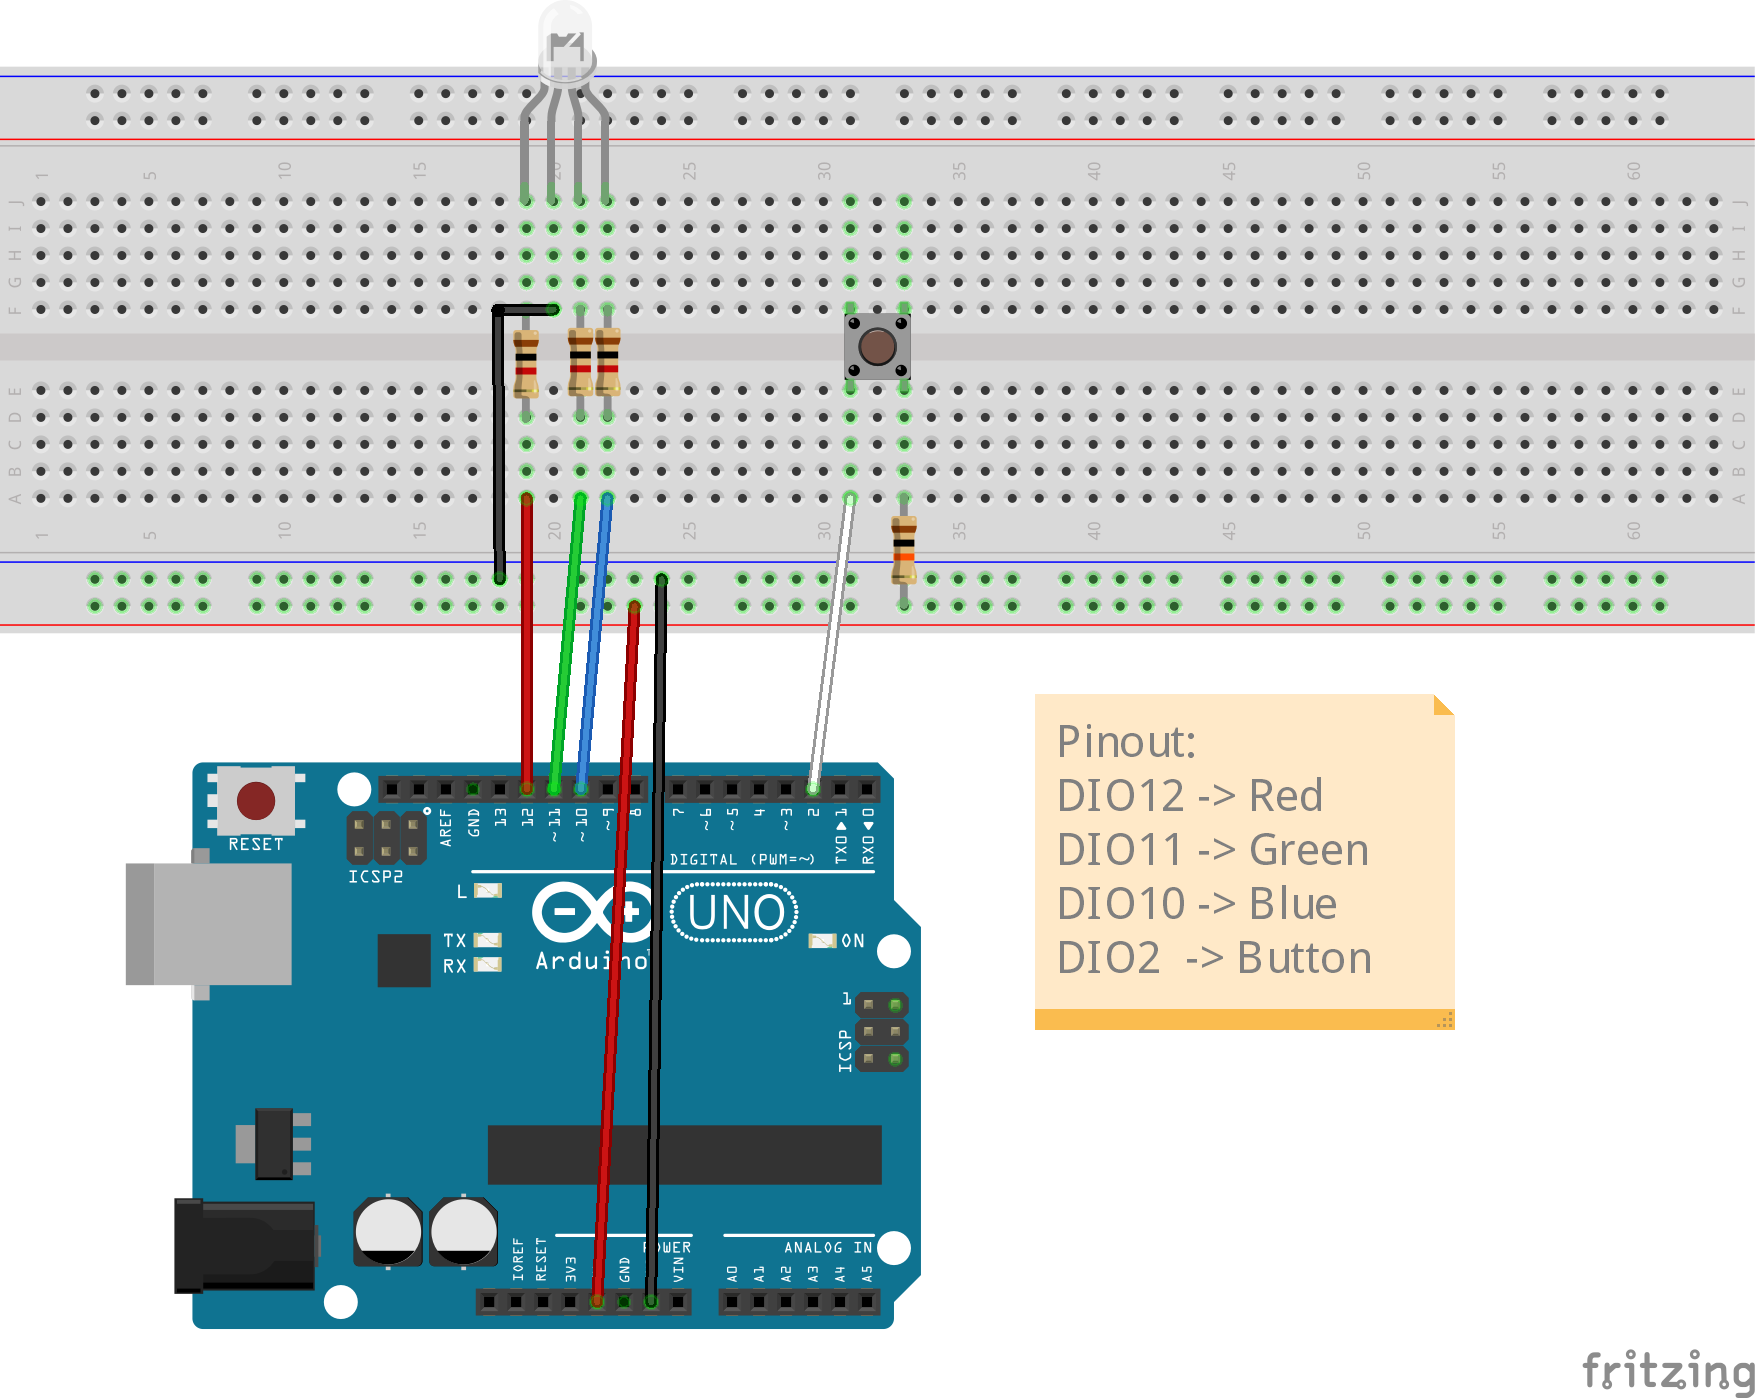
\includegraphics[]{p1_rgb_led_bb.png}
        \caption[]{The breadboard layout expected for this project}
        \label{fig:rgb_led_bb}
    \end{figure*}

    \begin{figure*}[ht!]
        \centering
        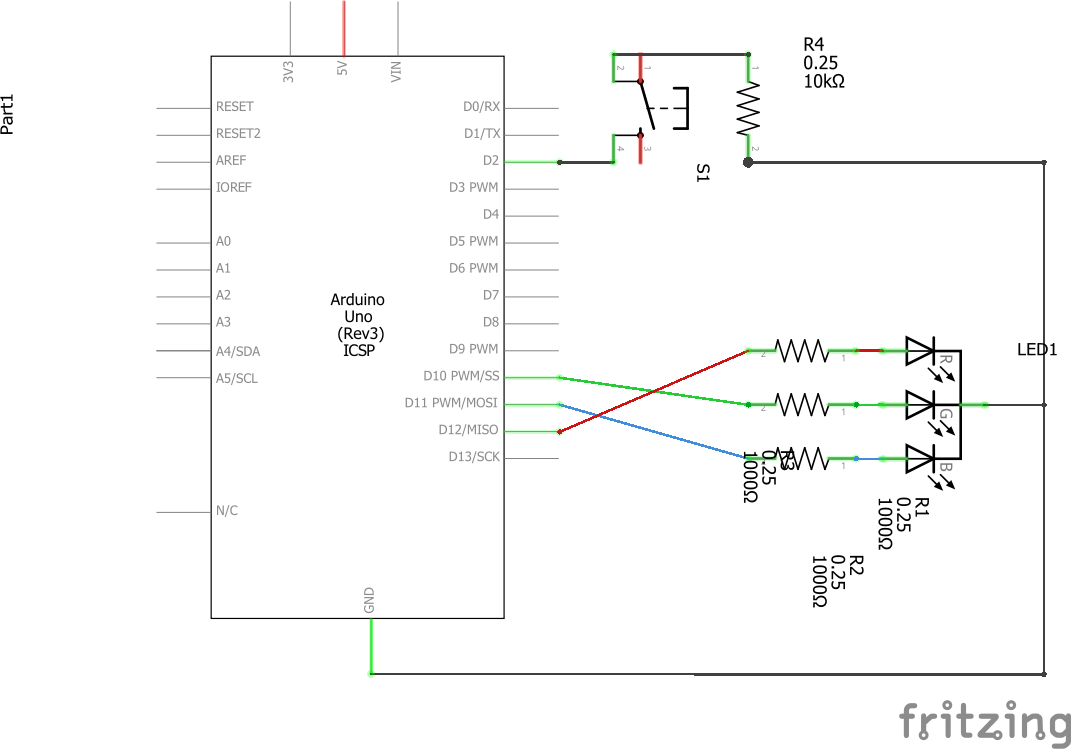
\includegraphics[]{p1_rgb_led_sch.png}
        \caption{The schematic layout expected for this project}
        \label{fig:rgb_led_sch}
    \end{figure*}

    \subsection*{Arduino Code}

    The student should have a well-organized and commented Arduino code for their project. 
    The code should have multiple functions including \lstinline[language=C++, style=mystyle]{void setup()} and \lstinline[language=C++, style=mystyle]{void loop()} along with their own LED implementations. 
    At least one of the LED functions must include a loop of somekind - either a for-loop or a while-loop that controls the LED's behavior.
    Inside \lstinline[language=C++, style=mystyle]{setup()}, the student should properly initialize the Arduino pins for inputs and outputs, with appropriately named variables for the pins. 
    Inside \lstinline[language=C++, style=mystyle]{loop()}, the student should have a switch-case statement that checks the LED mode and executes a different LED function for each mode.
    The same type of function can be called between different modes \emph{so long as they do different things}. 
    For example, LED mode 1 and 2 can both be \lstinline[language=C++, style=mystyle]{breathe()} so long as they do different colors.
    However, the student must have implemented at least three unique functions in their code.
    The easiest ones will most likely be: \lstinline[language=C++, style=mystyle]{staticColor()}, \lstinline[language=C++, style=mystyle]{breathe()}, and \lstinline[language=C++, style=mystyle]{rainbow()} - or some variation of that.
    It is up to the students to determine what they want to implement and how.

    The code below shows a basic solution to this project with four unique functions. 
    At the beginning, the pins are defined with clear variable names.
    The \lstinline[language=C++, style=mystyle]{#define} command is a pre-compiler instruction that essentially maps all calls of the specific variable name to the value.
    This is handy for declaring constant values in the program, such as pin numbers.

    In \lstinline[language=C++, style=mystyle]{setup()}, the Serial port is opened for debugging purposes.
    Then, the pins are suitably initialized as outputs and inputs.
    The button input pin is specified as a \lstinline[language=C++, style=mystyle]{INPUT_PULLUP} so that the microcontroller internally pulls the pin high instead of floating.
    When the button is pressed, the stronger pulldown resistor will for the pin to go LOW, creating a distinct signal that can be used for edge detection or easier button press detection.
    Here, students can implement an interrupt-based button debouncer and use that to switch the LED modes.
    If done properly, this would count as part of the extra credit.
    
    In \lstinline[language=C++, style=mystyle]{loop()}, the button input is first checked by determining if the button input pin is being pulled LOW by being pressed.
    If the button is pressed, then the LED mode is checked to see if it is the last mode specified by \lstinline[language=C++, style=mystyle]{MAX_LED_FUNCS}.
    If it is the last mode, the counter is reset otherwise, it is incremented.
    A switch-case statement checks the \lstinline[language=C++, style=mystyle]{ledMode} value and executes a specific function based on the value. The \lstinline[language=C++, style=mystyle]{default} case is present as an implicit fifth LED mode to do nothing and implicitly turn off the LEDs. 
    \emph{This can count as a unique function if implemented properly.}
    At the bottom of the function is a set of statements to reset the LED state to OFF between state function executions.
    
    \lstinline[language=C++, style=mystyle]{breathe()} uses two for-loops to linearly increase the LED's brightness from OFF to FULL to OFF again.
    The boolean parameters in the function call determine which LEDs are lit during this function allowing users to breathe either Red, Green, Blue, or White, as they desire.
    To make the effect more apparent, a \lstinline[language=C++, style=mystyle]{delay()} call is at the bottom of the function to slow the code execution down.

    \lstinline[language=C++, style=mystyle]{breatheSine()} uses the same principle as \lstinline[language=C++, style=mystyle]{breathe()} but uses a sine wave to accomplish the effect.
    By incrementing from 0-180 degrees, the light is brightened and dimmed in a sinusoidal fashion.
    As before, the boolean parameters in the function call determine which LEDs are lit, allowing for different color combinations.

    \lstinline[language=C++, style=mystyle]{rainbow()} builds upon the previous function by cycling all three LEDs in a sinusoidal fashion, but 120 degrees out of phase and shift so the wave amplitudes lie between 0 and 2.
    This creates a three-phase system that will cycle through most of the color combinations, except black and white.
    When running, three colored LEDs should clearly get brighter and darker and appear to be ``chasing'' each other around the diode.

    Finally, \lstinline[language=C++, style=mystyle]{staticColor()} just brightens an LED to a constant color and instensity specified in the function arguments.
    There is a delay at the end of the function to slow down the program execution and allow the program to better detect a button press and increment the LED mode.

    \pagebreak
    \lstinputlisting[language=C++, style=mystyle]{../../../src/projects/project_1_rgb_led/project_1_rgb_led.ino}
\end{document}
